% Introduction
\section{Introduction}

%%%%%%

% Cite:
% Wireless sensor networks	#yick2008wireless
% Mobile campus networks 	#hernandez2005comparative
% Mobile gaming community	#cunningham2002optimizing
% Energy-efficient network	#jones2001survey
% Internet of things 			#qin2014software
% Connectivity  			#moscibroda2006complexity
% Density					#wang2015connectivity

% The cite of the existing algorithms are listed in related work

%%%%%%

% Paper Logical Flow
% P1-P2 Background
% P3-P6 motivation
% P7-P11 contribution
% P12 structure

% P1:    
% Define realistic network
% General background
% The situation&scenario our research applies to
The growing interest in the Internet of Things (IoT) has resulted 
in a number of wide-area deployments of wireless networks \cite{qin2014software},
such as wireless sensor networks \cite{yick2008wireless}, mobile campus networks 
\cite{hernandez2005comparative}, mobile gaming community \cite{cunningham2002optimizing}, etc.
All these realistic networks possess multi-hop and large-scale characteristics.

% P2: 
% Why NB problem is related and important to the background in P1  
% Define what is neighbor and what is neighbor discovery problem
% A brief introduction of the existing works and explain deterministic and probabilistic with one sentence each
Neighbor discovery is a fundamental step of constructing a wireless network, based on 
which the network can perform further functions such as routing and broadcasting.
The primary goal is for each node in the network to discover the nodes in its radio sensing range 
with a one-hop communication, which are called neighbors. 
A number of existing methods \cite{dutta2008practical, kandhalu2010u,
bakht2012searchlight, sun2014hello, chen2015heterogeneous,
wang2015blinddate, qiu2016talk, mcglynn2001birthday,
vasudevan2009neighbor, you2011aloha, song2014probabilistic} have been proposed 
to deal with neighbor discovery, some of which are based on deterministic techniques, 
those turn on the radio with deterministic sequences,
while others are probabilistic approaches, those turn on the radio with different probabilities.


% P3:
% Crucial problem:  collision issue in a partially-connected network
% What is a practical network model and define what is a partially-connected network
Despite extensive research, neighbor discovery in a realistic network remains an open problem.
The key obstacle is the collision condition in such networks.
In any large-scale network, each node is only able to sense their neighbors
if their Euclidean distance is within a specific threshold 
based on received signal strength \cite{moscibroda2006complexity, wang2013gaussian, wang2015connectivity}.  
We call this multi-hop wireless network connectivity as \emph{partially-connected}.


% P4: 
% What issues will occur, if transferring the deterministic methods to the partially-connected network
% On the one hand,
On the one hand, the deterministic approaches only deal with the neighbor discovery problem for any two nodes.
When applied to a multiple node scenario, they are unable to solve the collision issue when two or more neighbors are transmitting simultaneously. As such they are not applicable in any large-scale realistic network.


% P5:
% What issues will occur, if transferring the probabilistic methods to the partially-connected network
% On the other hand,
On the other hand, probabilistic approaches can work with multiple nodes discovery. But, they are only ideal if
the network is fully-connected: the topology of the network is a complete graph. 
Therefore in large-scale networks where the nodes maybe partially-connected,  
the probability adopted in these approaches are not accurate and thus unable to reduce collision efficiently. 
To our knowledge, no relevant research focused on the neighbor discovery problem in the large-scale networks 
where nodes are partially-connected.


% P6: 
% Summarize our initiative insight
Our insight is to consider the entire distribution of the nodes in the network,
since in a wireless network the distribution of 
nodes, and their deployment play a vital role in determining the intrusion 
detection capability of a communication device.

% P7:
% Our solution/contribution : we propose Alano algorithm based on the distribution of nodes for the partially-connected networks
In this paper, we propose Alano\footnote{Alano is the god of luck in Greek mythology.}, to overcome the previously encountered problems. 
Alano is a nearly optimal probability based algorithm to discover neighbors in large-scale networks. 
As studied in \cite{wang2013gaussian} , the nodes in wireless sensor networks are likely to 
follow a uniform or a Gaussian distribution as showed in Fig. \ref{distribution}.
depending on the specific network applications, which is considered in our proposed algorithm.

 
 \begin{figure}[!t]
\centering
\subfigure[uniform distribution]{\includegraphics[width=1.7in]{./Figure/uniform.eps}}
\vspace{0.03in}
\subfigure[Gaussian distribution]{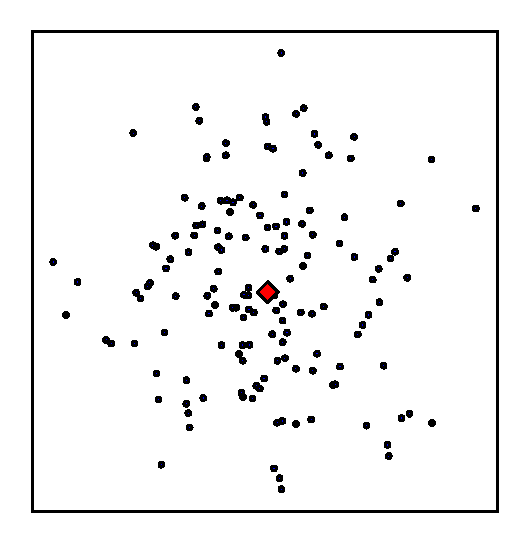
\includegraphics[width=1.7in]{./Figure/normal.eps}}
\caption{WSN deployments following uniform and Gaussian distribution.}
\label{distribution}
%\vspace{-0.2in}
\end{figure}


% P8: 
% A special type of partially-connected networks: energy-efficient network
In addition, among the large-scale networks, there is a specific 
type called energy-efficient network \cite{jones2001survey}.
Wireless sensor networks are typically energy-efficient networks that all the sensor nodes have to adhere to 
strict power control to prolong its lifetime\cite{dunkels2011contikimac}.
A duty cycle mechanism: measuring the amount of time the radio is turned on, is 
utilized to raise the power-awareness of the nodes in the network.
Corresponding to this the neighbor discovery process 
needs adjustments to balance between energy-efficiency and low-latency.


% P9: 
% For energy-efficient networks, we propose RDS-Alano in global duty cycle scenario 
% and TP-Alano in the local duty cycle scenario.
For energy-efficient networks, we design deterministic methods
to synchronize the wake up time slots between the neighbors to achieve a lower latency bound.
Specifically, We propose RDS-Alano algorithm for symmetric energy-efficient networks, where 
all the nodes share identical duty cycles $\theta$ and, TP-Alano for
asymmetric energy-efficient networks where each node possesses a separate duty cycle $\theta_i$. 


% P10:
% Simulation results support our high performance
Our simulation shows that our proposed algorithm, Alano,
hold provides significant benefits compared to other state-of-the-art methods.
Based on evaluations of speed, quality, scalability and robustness, 
Alano achieves 31.35\% to 32.32\% lower latency
and has a higher discovery rate during neighbor discovery, regardless if scenario is symmetric or asymmetric; uniform or Gaussian distribution.
In other work, when the number of nodes increases and the network becomes denser, however 
Alano still keeps its high performance. 


% P11:
% Contribution summarize
The main contributions of this paper are summarized as follows:
\begin{itemize}
\item[1)] We consider the distribution of nodes and propose Alano, 
a low-latency algorithm to achieve neighbor discovery in a large-scale realistic network.
\item[2)] We propose a Relaxed Difference Set based Alano algorithm (RDS-Alano) 
to achieve low-latency neighbor discovery process in the symmetric energy-efficient networks. 
\item[3)] We propose a Traversing Pointer based Alano algorithm (TP-Alano) to
achieve low-latency neighbor discovery process in the asymmetric energy-efficient networks. 
\end{itemize}


% P12:
% Remaining structure
The remainder of the paper is organized as follows.
The next section highlights related work and 
emphasis some gaps in existing research.
Some notations and definitions as well as the system model are given in Section \ref{sectionmodel}. 
We analyze the node's expected number of neighbors and 
propose Alano algorithm in \ref{PCN} as a foundation.
Section \ref{EEN} describes the RDS-Alano algorithm for 
symmetric scenario and TP-Alano algorithm for asymmetric scenario 
in energy-efficient networks.
We have conducted extensive simulations, and the results are shown in Section
\ref{Evaluation}. Finally, we conclude the paper in Section
\ref{Conclusion}.

\endsection{Introduction}



